\section{Correlation Functions}
Today is very exciting because we will study our first observables in QFT! We will study \emph{correlation functions}, which are important observables in not just QFT, but also QM, SM, CM\ldots

A type of correlation function we will consider is a two-point function of our scalar field:
\begin{equation}
    \bra{0}\hat{\phi}(t_1, \v{x}_1)\hat{\phi}(t_2, \v{x}_2)\ket{0}
\end{equation}
This object measures the correlation between two different points (measuring the correlations of the fluctuations in the quantum field at different points in spacetime); it is like a joint probability.

\subsection{The Utility of Correlation Functions}
These are related to many observables; for example, in linear response theory, two-point functions are related to observables like susceptibilities, conductivities, etc. For example, in Ohm's law, we study the linear response the current to an electric field:
\begin{equation}
    \v{J} = \sigma\v{E}
\end{equation}
with $\sigma$ the conductivity. In a quantum system, $\sigma$ is related to the two-point function of a current operator:
\begin{equation}
    \sigma \sim \avg{\hat{\v{J}}\hat{\v{J}}}.
\end{equation}
This will only become obvious later, when we introduce the path integral. For now, we just consider it as an example.

Another example comes from particle physics. Scattering amplitudes (the S-matrix) can be obtained from correlation functions, using what is known as the ``LSZ formula''. We will see this soon!

\subsection{Symmetry Constraints on Correlation Functions}
\subsubsection*{Translations}
Translation invariance implies that the correlators only depend on the differences between coordinates. Let us show this:
\begin{equation}
    \bra{0}\hat{\phi}(t_1, \v{x}_1)\hat{\phi}(t_2, \v{x}_2)\ket{0} = \bra{0}\hat{\phi}(t_1, \v{x}_1) e^{i(\hat{H}t_2 + \hat{\v{P}}s\cdot\v{x}_2)}\phi(0, 0)e^{-i(\hat{H}t_2 + \hat{\v{P}}\cdot\v{x})}\ket{0}
\end{equation}
Now, for the free scalar field the vacuum is translation-invariant, and that it is annihilated by the Hamiltonian:
\begin{equation}
    \hat{\v{P}}\ket{0} = 0, \quad \hat{H}\ket{0} = 0.
\end{equation}
This allows us to write:
\begin{equation}
    \bra{0}\hat{\phi}(t_1, \v{x}_1)\hat{\phi}(t_2, \v{x}_2)\ket{0} = \bra{0}e^{-i(\hat{H}t_2 + \hat{\v{P}}\cdot\v{x})} \hat{\phi}(t_1, \v{x}_1)e^{i(\hat{H}t_2 + \hat{\v{P}}\cdot\v{x})}\hat{\phi}(0, \v{0})\ket{0}
\end{equation}
Then, using the conjugation to translate the first field:
\begin{equation}
    \bra{0}\hat{\phi}(t_1, \v{x}_1)\hat{\phi}(t_2, \v{x}_2)\ket{0} = \bra{0}\hat{\phi}(t_1 - t_2, \v{x}_1 - \v{x}_2)\hat{\phi}(0, \v{0})\ket{0}
\end{equation}
Thus we see that the correlator only depends on the difference between the spacetime coordinates. Note we have used two things here; the translation invariance of the vacuum, as well as the fact that $[\hat{H}, \hat{\v{P}}] = 0$ (else we cannot nontrivially place them in the same exponential!) Note that this is not always true, for example this symmetry is broken in some condensed matter systems.

This motivates the following definition:
\begin{equation}
    G_W(x^\mu) = \bra{0}\hat{\phi}(t, \v{x})\hat{\phi}(0, \v{0})\ket{0}
\end{equation}
This is known as a \emph{Wightman function}. It is a Green's function.

\subsubsection*{Lorentz Invariance}
We assume now that:
\begin{equation}
    U(\Lambda)\ket{0} = \ket{0}.
\end{equation}
This implies that:
\begin{equation}
    G_W(x^\mu) = \bra{0}U(\Lambda)^{-1}\hat{\phi}(x^\mu)U(\Lambda)U(\Lambda)^{-1}\hat{\phi}(0)U(\Lambda)\ket{0}
\end{equation}
Then using the transformation property of a scalar field:
\begin{equation}
    G_W(x^\mu) = \bra{0}\hat{\phi}(\Lambda^{-1}x)\hat{\phi}(0)\ket{0} = G_W(\Lambda^{-1}x)
\end{equation}
Thus, the Wightman function is invariant under a Lorentz transformation between the coordinates. For rotations, this implies for example that the correlation between two points is the same if I look at two points rotated. More generally, this implies that the Wightman fucntion can only depend on a Lorentz invairance combination of $x^\mu$s, i.e. it can only depend on $x^2 = \eta_{\mu\nu}x^\mu x^\nu$:
\begin{equation}
    G_W(x^\mu) = G_W(x^2).
\end{equation}
So with very little work, we have shown the 2-point functions only depend on a single variable (as opposed to the four variables $t, x_1, x_2, x_3$). This is the power of symmetry. Note that this result holds for any quantum field theory (interacting, or free) with this symmetry.

\subsection{2-Point Correlator for the Free Scalar Field Theory}
Let us work out the correlation functions explicitly. 

We defined:
\begin{subequations}
    \begin{align}
    a_\v{k} &= (\e_\v{k}\hat{\phi}_\v{k} + i\hat{\Pi}_\v{k})
    \\ a_\v{k}^\dag &= (\e_\v{k}\hat{\phi}_\v{-k} - i\hat{\Pi}_\v{-k})
    \end{align}
\end{subequations}
where we note the redefinition such that the normalization of the momentum eigenstates will be Lorentz Invariant (see HW2):
\begin{equation}
    \bra{0}a_\v{k}a_\v{k}^\dag\ket{0} = 2\e_{\v{k}}(2\pi)^d\delta^d(\v{k} - \v{k}')
\end{equation}
with $\e_\v{k} = \sqrt{\v{k}^2 + m^2}$. We introduced these operators because they solved the problem, in the sense that they have trivial time evolution:
\begin{subequations}
    \begin{align}
    e^{i\hat{H}t}a_\v{k}^\dag e^{-i\hat{H}t} &= e^{i\e_{\v{k}}t}a^\dag_\v{k}
    \\ e^{i\hat{H}t}a_\v{k} e^{-i\hat{H}t} &= e^{-i\e_{\v{k}}t}a_\v{k}
    \end{align}
\end{subequations}
which is worked out from $[\hat{H}, a_\v{k}^\dag] = \e_\v{k}a_\v{k}^\dag$. Then, from this we know the time evolution of $\phi_\v{k}$:
\begin{equation}
    \phi_\v{k} = \frac{1}{2\e_\v{k}}(a_\v{k} + a^\dag_{-\v{k}})
\end{equation}
Using this, let's work out the Wightman function:
\begin{equation}
    G_W(x^\mu) = \bra{0}\hat{\phi}(t, \v{x})\hat{\phi}(0, 0)\ket{0} = \int \frac{d^dk}{(2\pi)^d}\frac{d^dk'}{(2\pi)^d}e^{i\v{k} \cdot \v{x}}\bra{0}\phi_\v{k}(t)\phi_{\v{k}'}(0)\ket{0}
\end{equation}
Only the raising term will contribute for the $\phi_{\v{k}'}(0)$, and only the (time-evolved) lowering term will contribute for $\phi_\v{k}(t)$, thus:
\begin{equation}
    \begin{split}
        G_W(x^\mu) &= \int d^dk d^dk' \frac{e^{i(\v{k} \cdot \v{x} - \e_\v{k}t)}}{4\e_\v{k}\e_{\v{k}'}} \bra{0}a_\v{k}a^\dag_{-\v{k}'}\ket{0} 
        \\ &= \int d^dk d^dk' \frac{e^{i(\v{k} \cdot \v{x} - \e_\v{k}t)}}{4\e_\v{k}\e_{\v{k}'}} (2\pi)^d \delta^d(\v{k} + \v{k}')2\e_{\v{k}}
        \\ &= \int \frac{d^dk}{(2\pi)^d}\frac{e^{i(\v{k} \cdot \v{x} - \e_\v{k}t)}}{2\e_\v{k}}
    \end{split}
\end{equation}
This is a bit tedious to compute in general (on HW3), but for now we consider a special case where we can solve this live in closed form. Two simplifications; we take $d=1$ and we will set $m = 0$:
\begin{equation}
    G_W(x^\mu) = \int \frac{dk}{2\pi}\frac{e^{i(kx - \abs{k}t)}}{2\abs{k}}
\end{equation}
We will make this easier for ourselves by computing the time-derivative of the Wightman function, which will cancel out the $\abs{k}$ appearing in the denominator:
\begin{equation}
    \p_t G_W(x^\mu) = -\frac{i}{2}\int \frac{dk}{2\pi}e^{i(kx - \abs{k}t)}
\end{equation}
Since there's an absolute value, let us separate the integral out into the $k > 0$ and $k < 0$ part:
\begin{equation}
    \p_t G_W(x^\mu) = -\frac{i}{2}\left[\int_0^\infty \frac{dk}{2\pi}e^{ik(x - t)} + \int_{-\infty}^0 e^{ik(x + t)}\right]
\end{equation}
These integrals look simple, but also don't look like they want to converge... which tells us these observables are a little subtle. In order to make them converge, we evaluate the function at $t - i\e$ for $\e$ small:
\begin{equation}
    \begin{split}
        \p_t G_W(t - i\e, \v{x}) &= -\frac{i}{2}\left[\int_0^\infty \frac{dk}{2\pi}e^{ik(x - (t-i\e))} + \int_{-\infty}^0 e^{ik(x + (t-i\e))}\right]
        \\ &= -\frac{i}{4\pi}\left[ \left.\frac{e^{ik(x - (t-i\e))}}{i(x - (t - i\e))} \right|_0^\infty +  \left.\frac{e^{ik(x + (t-i\e))}}{i(x + (t - i\e))} \right|_0^\infty \right]
        \\ &= - \frac{i}{4\pi}\left[\frac{-1}{i(x - (t-i\e))} + \frac{1}{i(x + (t-i\e))}\right]
        \\ &= \frac{1}{4\pi}\left[\frac{x + (t - i\e) - [x - (t-i\e)]}{x^2 - (t-i\e)^2}\right]
        \\ &= \frac{1}{2\pi}\frac{t-i\e}{x^2 - (t - i\e)^2} 
        \\ &= -\frac{1}{4\pi}\p_t \log(x^2 - (t-i\e)^2)
    \end{split}
\end{equation}
In the numerator, we may take the $\e \to 0$ limit smoothly always, but in the denominator singularities can occur, so in general we need to be careful about taking this limit.

Thus; up to a constant:
\begin{equation}
    \boxed{G_W(x^\mu) = -\frac{1}{4\pi}\log(x^2 - t^2)}
\end{equation}
Note that this is indeed Lorentz invariant, as it only depends on $x_\mu x^\mu$! It is also interesting to plot, where we see that it is sharply peaked on the lightcone.

\begin{figure}[htbp]
    \centering
    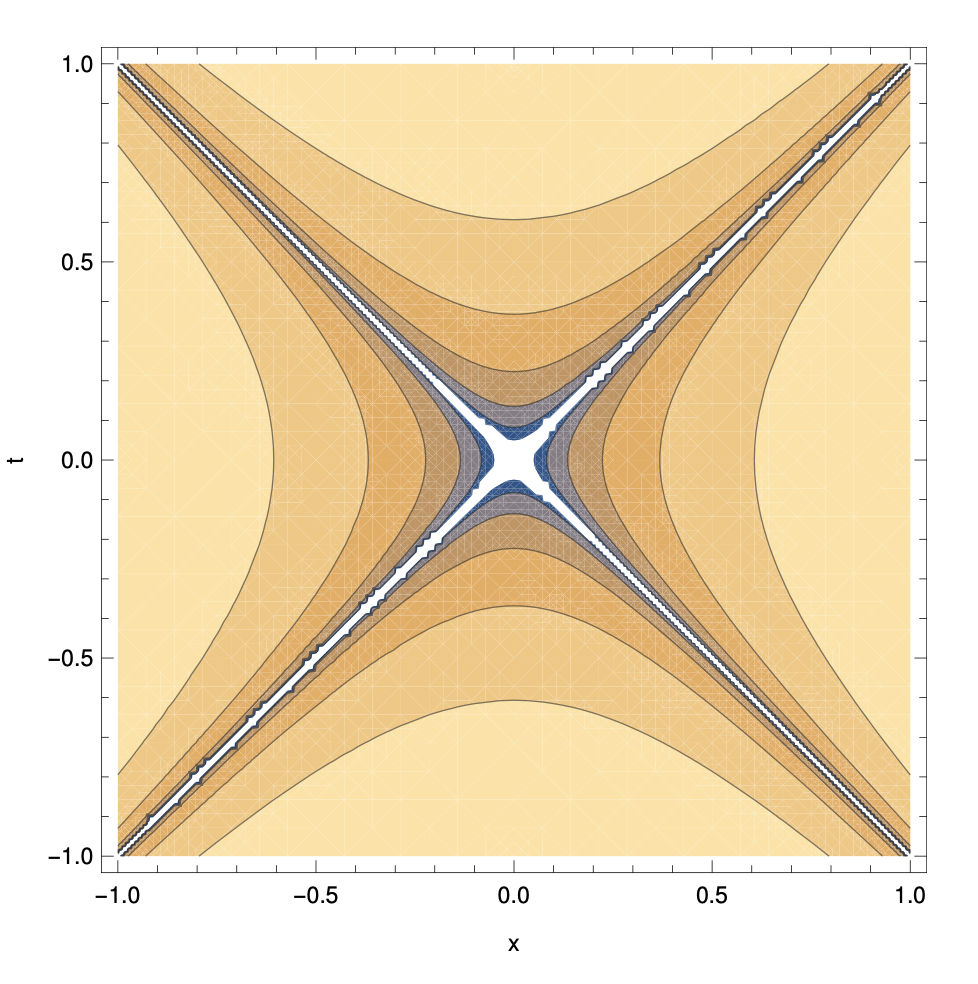
\includegraphics[scale=0.5]{Lectures/Figures/logt2x2.png}
    \caption{Plot of $\log(x^2 - t^2)$, courtesy of Luca.}
    \label{fig-logt2x2}
\end{figure}

This should not surprise us; the massless free scalar propogates at the speed of light, hence the field is very correlated with itself on the lightcone.

Remark for the formally minded: In an axiomatic approach to QFT, real-time correlators are defined by $\e \to 0$ limits of Wick rotated (analytic continuations) to imaginary time versions of the correlators, and there are perscriptions on how to handle those limits/navigate around branch cuts.

\subsection{2-Point correlator for the Free Scalar Field Theory: Momentum Space}
Restoring $m \neq 0$ and general $d$, one can evaluate the Fourier transform of the correlator of $G_W$:
\begin{equation}
    \begin{split}
        G_W(\omega, \v{k}) &= \int dt d^dx e^{-i\v{k}\cdot\v{x} - i\omega t}G_W(t, \v{x})
        \\ &= \int \frac{dtd^dxd^dk'}{(2\pi)^d}e^{i(\v{k}' - \v{k})\cdot \v{x}} e^{i(\omega - \e_{\v{k}'})t}\frac{1}{2\e_\v{k}}
    \end{split}
\end{equation}
The $x$ integral is simple and sets $\v{k'} = \v{k}$. We are then left with:
\begin{equation}
    G_W(\omega, \v{k}) = \int dt \frac{e^{i(\omega - \e_{\v{k}})t}}{2\e_\v{k}} = \frac{2\pi\delta(\omega - \e_\v{k})}{2\e_\v{k}}
\end{equation}
Thus:
\begin{equation}
    \boxed{G_W(\omega, \v{k}) = \frac{2\pi\delta(\omega - \e_\v{k})}{2\e_\v{k}}}
\end{equation}
which tells us that the Green's function only fires/resonates when $\omega = \e_\v{k}$. When we evaluated the position-space Green's function, we had the Lorentz invariance constraint. We might expect this for the momentum space version, namely:
\begin{equation}
    G_W(p^\mu) = G_W(\Lambda p^\mu).
\end{equation}
It does not look manifestly Lorentz invariant, but it is, and we will show this.

\subsection{The Feynman Correlator}
We now consider:
\begin{equation}
    G_F(t, \v{x}) = \bra{0}\mathcal{T}\set{\hat{\phi}(t, \v{x})\hat{\phi}(0, 0)}\ket{0}
\end{equation}
where $\mathcal{T}\{\cdot\}$ denotes the time-ordering operation. In other words:
\begin{equation}
    G_F(t, \v{x}) = \mathcal{T}\set{\hat{\phi}(t, \v{x})\hat{\phi}(0, \v{0})} = \Theta(t)\bra{0}\hat{\phi}(t, \v{x})\hat{\phi}(0, \v{0})\ket{0} + \Theta(-t)\bra{0}\hat{\phi}(0, \v{0})\hat{\phi}(t, \v{x})\ket{0}.
\end{equation}
With $\Theta$ the step function. This is still a measure of correlation between two points, but slightly modified. Evaluating this:
\begin{equation}
    G_F(t, \v{x}) = \Theta(t)\int \frac{d^dk}{(2\pi)^d}\frac{e^{i(\v{k} \cdot \v{x} - \e_\v{k}t)}}{2\e_\v{k}} + \Theta(-t)\int \frac{d^dk}{(2\pi)^d}\frac{e^{-i(\v{k} \cdot \v{x} - \e_\v{k}t)}}{2\e_\v{k}}.
\end{equation}
Let's compute the Fourier transform of this expression:
\begin{equation}
    \begin{split}
        G_F(\omega, \v{k}) &= \int dt d^dx e^{i(\omega t - \v{k} \cdot \v{x})}G_F(x^\mu)
        \\ &= \int dt \Theta(t)\frac{e^{i(\omega - \e_{\v{k}})t}}{2\e_\v{k}} + \Theta(-t)\frac{e^{i(\omega + \e_{\v{k}})t}}{2\e_\v{k}}
        \\ &= \int_0^\infty dt \frac{e^{i(\omega - \e_{\v{k}} + i\e)t}}{2\e_\v{k}} + \int_{-\infty}^0dt \frac{e^{i(\omega + \e_{\v{k}} - i\e)t}}{2\e_\v{k}}
        \\ &= \frac{1}{2\e_\v{k}}\left[\left.\frac{e^{i(\omega - \e_k + i\e)}}{i(\omega - \e_k + i\e)}\right|_0^\infty +\left.\frac{e^{i(\omega + \e_k - i\e)t}}{i(\omega + \e_k - i\e)t}\right|_{-\infty}^0\right]
        \\ &= \frac{1}{2\e_\v{k}}\left[\frac{-1}{i(\omega - \e_\v{k} + i\e)} + \frac{1}{i(\omega + \e_\v{k} - i\e)}\right]
        \\ &= \frac{i}{\omega^2 - (\e_\v{k} - i\e)^2}
        \\ &= \frac{i}{\omega^2 - \e_\v{k}^2 + i\tilde{\e}}
        \\ &= \frac{-i}{p^2 + m^2 - i\tilde{\e}}
    \end{split}
\end{equation}
We have again introduced the appropriate $i\e$s in order to avoid the divergences. Note that later on we will see a physical application of this; in the context of unstable particles, we have a decay that introduces some broadening of the linewidths. Also in the last lines we redefine $\tilde{\e}$ as we don't care what the small factor is, only its sign. Thus:
\begin{equation}
    \boxed{G_F(\omega, \v{k}) = \frac{-i}{p^2 + m^2 - i\tilde{\e}}}
\end{equation}
Note that this is qualitatively pretty different from the Wightman function; it does still diverge at $p^2 = -m^2$, but it is non-zero ``off-shell'', i.e. when $p^2 \neq -m^2$. Conversely, the Wightman function only fires on-shell. We will use this correlator all the time in the path integral formalism.